% !TeX root = algorithmik.tex

\section{Elementares über Graphen}


\begin{definition}
	Ein ungerichteter Graph ist ein Paar $G = (V,E)$, mit $V, E$ Mengen. $V$ heißt Menge von Knoten, $E$ heißt Menge von Kanten. Außerdem gibt es eine Funktion $i: E \rightarrow \mathcal{P}(V)$ mit $\mathcal{P}(V) = 2^V$ (Potenzmenge) und $0 < i(e) \leq 2$. $i$ gibt die Endpunkte einer Kante an.
	
	Ist $i(e) = \{ u, v \}$, so heißen $u, v$ Endpunkte von $e$. Ist $i(e_1) = i(e_2)$, so heißen $e_1, e_2$ parallel. Ist $|i(e)| = 1$, so heißt $e$ Schleife.
	
	Der Grad eines Knotens $v$, $grad(v)$, ist die Anzahl der Kanten, für die $v$ Endpunkt ist, wobei Schleifen doppelt gezählt werden. Ist $grad(v) = 0$, so heißt $v$ isoliert.
	
	Ein Graph heißt endlich, wenn $V$ und $E$ endlich sind.
\end{definition}


\begin{beispiel}
	\qquad
	\vspace{2mm}
	
	\begin{minipage}{8cm}
		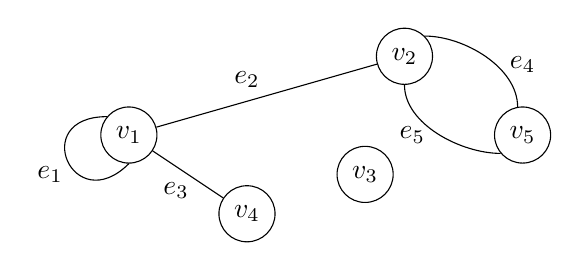
\begin{tikzpicture}
			\node (v4) at (2,0) [draw, shape=circle] {$v_4$};
			\node (v1) at (0.5,1) [draw, shape=circle] {$v_1$};
			\node (v3) at (3.5,0.5) [draw, shape=circle] {$v_3$};
			\node (v2) at (4,2) [draw, shape=circle] {$v_2$};
			\node (v5) at (5.5,1) [draw, shape=circle] {$v_5$};
			
			\draw(v4) -- (v1);
			\draw(v1) -- (v2);
			\draw(v1) -- (v1);
			\draw(v2.45) .. controls +(0:0.5) and +(90:0.5) .. (v5.100);
			\draw(v2.270) .. controls +(90:-0.5) and +(0:-0.5) .. (v5.220);
			\draw(v1.270) .. controls +(45:-1) and +(0:-1) .. (v1.140);
			
			\node (e1) at (-0.5, 0.5) { $e_1$ };
			\node (e2) at (2, 1.7) { $e_2$ };
			\node (e4) at (5.5, 1.9) { $e_4$ };
			\node (e5) at (4.1, 1) { $e_5$ };
			\node (e3) at (1.1, 0.3) { $e_3$ };
		\end{tikzpicture}
	\end{minipage}
	\begin{minipage}{5cm}	
	\begin{tabular}[t]{rl}
		$v_3$ & isoliert \\
		$e_4, e_5$ & parallel \\
		$e_1$ & Schleife \\
		$i(e_4) =$& $ \{ v_2, v_5 \} = i(e_5)$\\
		$grad(v_1) =$& $4$ \\
		$grad(v_2) =$& $3$ \\
	\end{tabular}
	\end{minipage}
\end{beispiel}


\begin{beispiel}
	Unendliche Graphen
	
	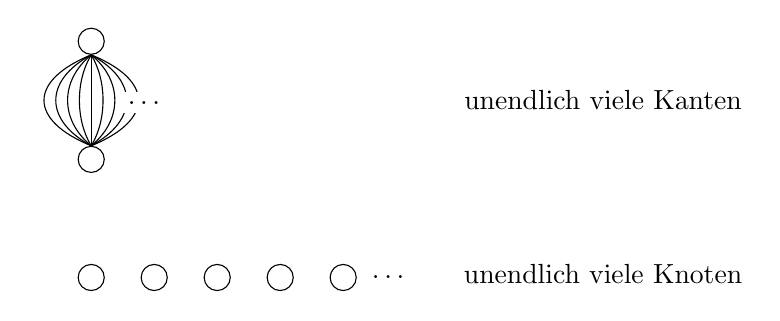
\begin{tikzpicture}
		\node (v1) at (0, 1.5) [draw, shape=circle] {};
		\node (v2) at (0, 0) [draw, shape=circle] {};
		
		\foreach \a in {-0.8, -0.6, -0.4, -0.2, 0, 0.2, 0.4, 0.6, 0.8}
			\draw (v1.south) .. controls (\a,1) and (\a, 0.5) .. (v2.north);
			
		\node (punkte) at (0.7, 0.72) [fill=white] {\dots};
		\node (bla) at (6.5, 0.76) {unendlich viele Kanten};
		
		\foreach \a in {0, 0.8, 1.6, 2.4, 3.2}
			\node at (\a, -1.5) [draw, shape=circle] {};
			
		\node (punkte2) at (3.8, -1.5) {\dots};
		\node (bla2) at (6.5, -1.45) {unendlich viele Knoten};
	\end{tikzpicture}
\end{beispiel}


\begin{bemerkung}
	In einem endlichen Graph ist die Anzahl der Knoten mit ungeradem Grad gerade.
\end{bemerkung}


\begin{beweis}
	Sei $V = \{ v_1, \dots, v_n \}$, dann ist $\sum_{i=1}^n grad(v_i) = 2 |E|$. Denn: starten wir mit $G = (V, \emptyset)$ und fügen die Kanten nacheinander ein, dann erhöht das Einfügen den Grad beider beteiligten Knoten um jeweils 1. Handelt es sich bei der Kante um eine Schleife, wir der Grad des Knotens um 2 erhöht.
	
	Seien o.E. $v_1 \dots v_j$ mit geradem Grad und $v_{j+1} \dots v_n$ mit ungeradem Grad. $\sum_{l=1}^j grad(v_l)$ ist eine gerade Zahl. Über alle Knoten summiert ergibt sich auch eine gerade Zahl $2|E|$.
	$$ 2|E| = \sum_{i=1}^n grad(v_i) = \underbrace{\sum_{i=1}^j grad(v_i)}_{gerade} + \underbrace{\sum_{i=j+1}^n \overbrace{grad(v_i)}^{ungerade}}_{gerade} $$
	Damit $\sum_{i=j+1}^n grad(v_i)$ gerade ist, muss die Anzahl dieser ungeraden Knoten gerade sein.
\end{beweis}


\begin{definition}
	Sei $G = (V,E)$ ein Graph. Sind $v_1, v_2$ die Endpunkte von $e$, so heißen $v_1, v_2$ benachbart. Ein Weg in G ist eine Folge von Kanten $e_1, e_2, \dots$, so dass gilt:
	\begin{enumerate}
		\item $\forall i$ gilt: $e_i, e_{i+1}$ haben einen gemeinsamen Endpunkt.
		\item ist $e_i$ keine Schleife und weder erste noch letzte Kante, so hat $e_i$ einen Knoten mit $e_{i-1}$ gemeinsam und den anderen mit $e_{i+1}$.
	\end{enumerate}
\end{definition}	


\begin{beispiel}
	\qquad
	\vspace{2mm}
	
	\begin{minipage}{4cm}
		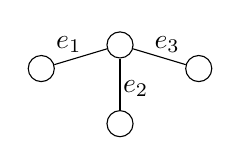
\begin{tikzpicture}
			\node (v1) at (0, -0.3) [draw, shape=circle] {};
			\node (v2) at (1, 0) [draw, shape=circle] {};
			\node (v3) at (2, -0.3) [draw, shape=circle] {};
			\node (v4) at (1, -1) [draw, shape=circle] {};
			
			\draw (v1) -- (v2);
			\draw (v2) -- (v3);
			\draw (v2) -- (v4);
			
			\node (l1) at (0.35, 0) {$e_1$};
			\node (l2) at (1.6, 0) {$e_3$};
			\node (l3) at (1.2, -0.55) {$e_2$};
			
		\end{tikzpicture}
	\end{minipage}
	\begin{minipage}{10cm}
		Ist $e_1, e_2, e_3$ ein Weg?
		
		\emph{1. ist erfüllt, 2. nicht $\Rightarrow$ kein Weg}
		 
		 $e_1, e_2, e_2, e_3$ ist ein Weg.
	\end{minipage}
\end{beispiel}


\begin{definition}
	Ein Weg wird auch dargestellt:
	\vspace{2mm}
	
	\begin{center}
		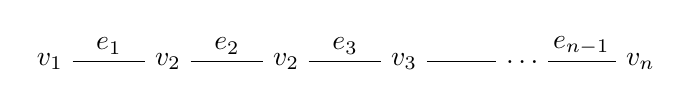
\begin{tikzpicture}
			\node (v1) at (0, 0) {$v_1$};
			\node (v2) at (1.5, 0) {$v_2$};
			\node (v22) at (3, 0) {$v_2$};
			\node (v3) at (4.5, 0) {$v_3$};
			\node (v4) at (6, 0) {$\dots$};
			\node (v5) at (7.5, 0) {$v_n$};
			
			\draw (v1) -- (v2);
			\draw (v2) -- (v22);
			\draw (v22) -- (v3);
			\draw (v3) -- (v4);
			\draw (v4) -- (v5);
			
			\node (l1) at (0.75, 0.2) {$e_1$};
			\node (l2) at (2.25, 0.2) {$e_2$};
			\node (l3) at (3.75, 0.2) {$e_3$};
			\node (l4) at (6.75, 0.2) {$e_{n-1}$};

		\end{tikzpicture}
	\end{center}
	
	In diesem Weg entspricht $e_2$ einer Schleife an $v_2$. Ist dieser abgebildete Weg endlich, so heißen $v_1$ Anfangspunkt und $v_n$ Endpunkt. Die Länge eines Weges ist gleich der Anzahl der Kanten, die er enthält.
	
	Ein Kreis (Zyklus) ist ein Weg, dessen Anfangspunkt und Endpunkt gleich sind. Ein Weg heißt einfach, wenn jeder Knoten höchstens einmal vorkommt. Ein Kreis der Länge $\ne 2$ heißt einfach, wenn jeder Knoten außer Anfangs- und Endpunkt höchstens einmal vorkommt.
\end{definition}


\begin{definition}
	Ein Graph $G = (V, E)$ heißt zusammenhängend, wenn es zwischen je zwei Knoten in $V$ einen Weg gibt, der sie verbindet, d.h. einer der Knoten ist Anfangspunkt und einer ist Endpunkt. 
	
	Es gibt für jeden Knoten $v$ der Menge $V$ einen Weg zu $v$ der Länge $0$.
\end{definition}